\documentclass[11pt,a4paper]{article}
\usepackage[margin=1in]{geometry}
\usepackage{amsmath,amssymb,amsthm}
\usepackage{bm}
\usepackage{hyperref}
\usepackage{graphicx}
\usepackage{caption}
\usepackage{listings}
\usepackage{xcolor}
\usepackage{float}
\usepackage{placeins}

% Graphics path
\graphicspath{{figures/}}

% Listings style
\lstdefinestyle{code}{%
  language=Python,
  basicstyle=\ttfamily\small,
  keywordstyle=\color{blue},
  commentstyle=\color{gray},
  stringstyle=\color{red!70!black},
  showstringspaces=false,
  breaklines=true,
  frame=single,
  numbers=left,
  numberstyle=\tiny, 
  numbersep=6pt,
  tabsize=4,
  columns=fullflexible
}

% Hyperref setup
\hypersetup{
  colorlinks=true,
  linkcolor=blue,
  citecolor=blue,
  urlcolor=blue
}

\title{Logistic Regression: A Practical Tutorial}
\author{Your Name}
\date{\today}

\begin{document}
\maketitle

\begin{abstract}
Logistic regression is a fundamental model for binary classification, widely used due to its interpretability and probabilistic outputs. This tutorial reviews the theory, provides practical tips, and offers a Python script to generate illustrative figures.
\end{abstract}

\section{Introduction}
Logistic regression models the conditional probability of a binary label given features. Unlike linear regression, it uses the sigmoid link to ensure outputs lie in $[0,1]$, making it well-suited for classification and calibrated probability estimation. Common applications include risk prediction, medical diagnosis, and click-through-rate modeling.

\section{Theory and Formulas}
Let $\bm{x} \in \mathbb{R}^d$ and $y \in \{0,1\}$. The model is
\begin{equation}
  p(y=1\mid \bm{x}) = \sigma(z), \quad z = w_0 + \bm{w}^\top \bm{x}, \quad \sigma(t) = \frac{1}{1+e^{-t}}.
\end{equation}
Equivalently, the log-odds (logit) is linear: $\log \frac{p}{1-p} = w_0 + \bm{w}^\top \bm{x}$.

Given $n$ i.i.d. samples $\{(\bm{x}_i,y_i)\}_{i=1}^n$, the negative log-likelihood (binary cross-entropy) is
\begin{equation}
  \mathcal{L}(\bm{w},w_0) = -\sum_{i=1}^n \left[ y_i \log p_i + (1-y_i)\log (1-p_i)\right],\quad p_i = \sigma(w_0+\bm{w}^\top\bm{x}_i).
\end{equation}
The gradient is
\begin{equation}
  \nabla_{\bm{w}}\, \mathcal{L} = \sum_{i=1}^n (p_i - y_i)\,\bm{x}_i, \qquad \frac{\partial \mathcal{L}}{\partial w_0} = \sum_{i=1}^n (p_i - y_i).
\end{equation}
With $\ell_2$-regularization (ridge), add $\tfrac{\lambda}{2}\lVert \bm{w}\rVert^2$ to the loss to reduce overfitting.

The decision boundary for threshold $0.5$ is $\sigma(z)=0.5 \iff z = 0$, i.e., the hyperplane $w_0 + \bm{w}^\top\bm{x} = 0$.

\section{Applications and Tips}
\begin{itemize}
  \item Feature scaling helps optimization and interpretability of coefficients.
  \item Consider class imbalance: adjust decision threshold, use class weights, or resampling.
  \item Regularize to mitigate multicollinearity; $\ell_2$ is standard; $\ell_1$ promotes sparsity.
  \item Calibrated probabilities enable ranking and decision-making under costs.
  \item Inspect coefficients and odds ratios $e^{w_j}$ for interpretability.
\end{itemize}

\section{Python Practice}
Run the following script to generate figures used in this document. It has no exotic dependencies beyond NumPy and Matplotlib; it includes a simple logistic regression implementation to avoid version issues.
\begin{lstlisting}[style=code,caption={Python script to generate figures},label={lst:gen}]
\end{lstlisting}
You can also include the source directly:
\lstinputlisting[style=code,caption={gen\_logistic\_regression\_figures.py},label={lst:source}]{gen_logistic_regression_figures.py}

\section{Result}
Core illustrations are shown below.

\begin{figure}[H]
  \centering
  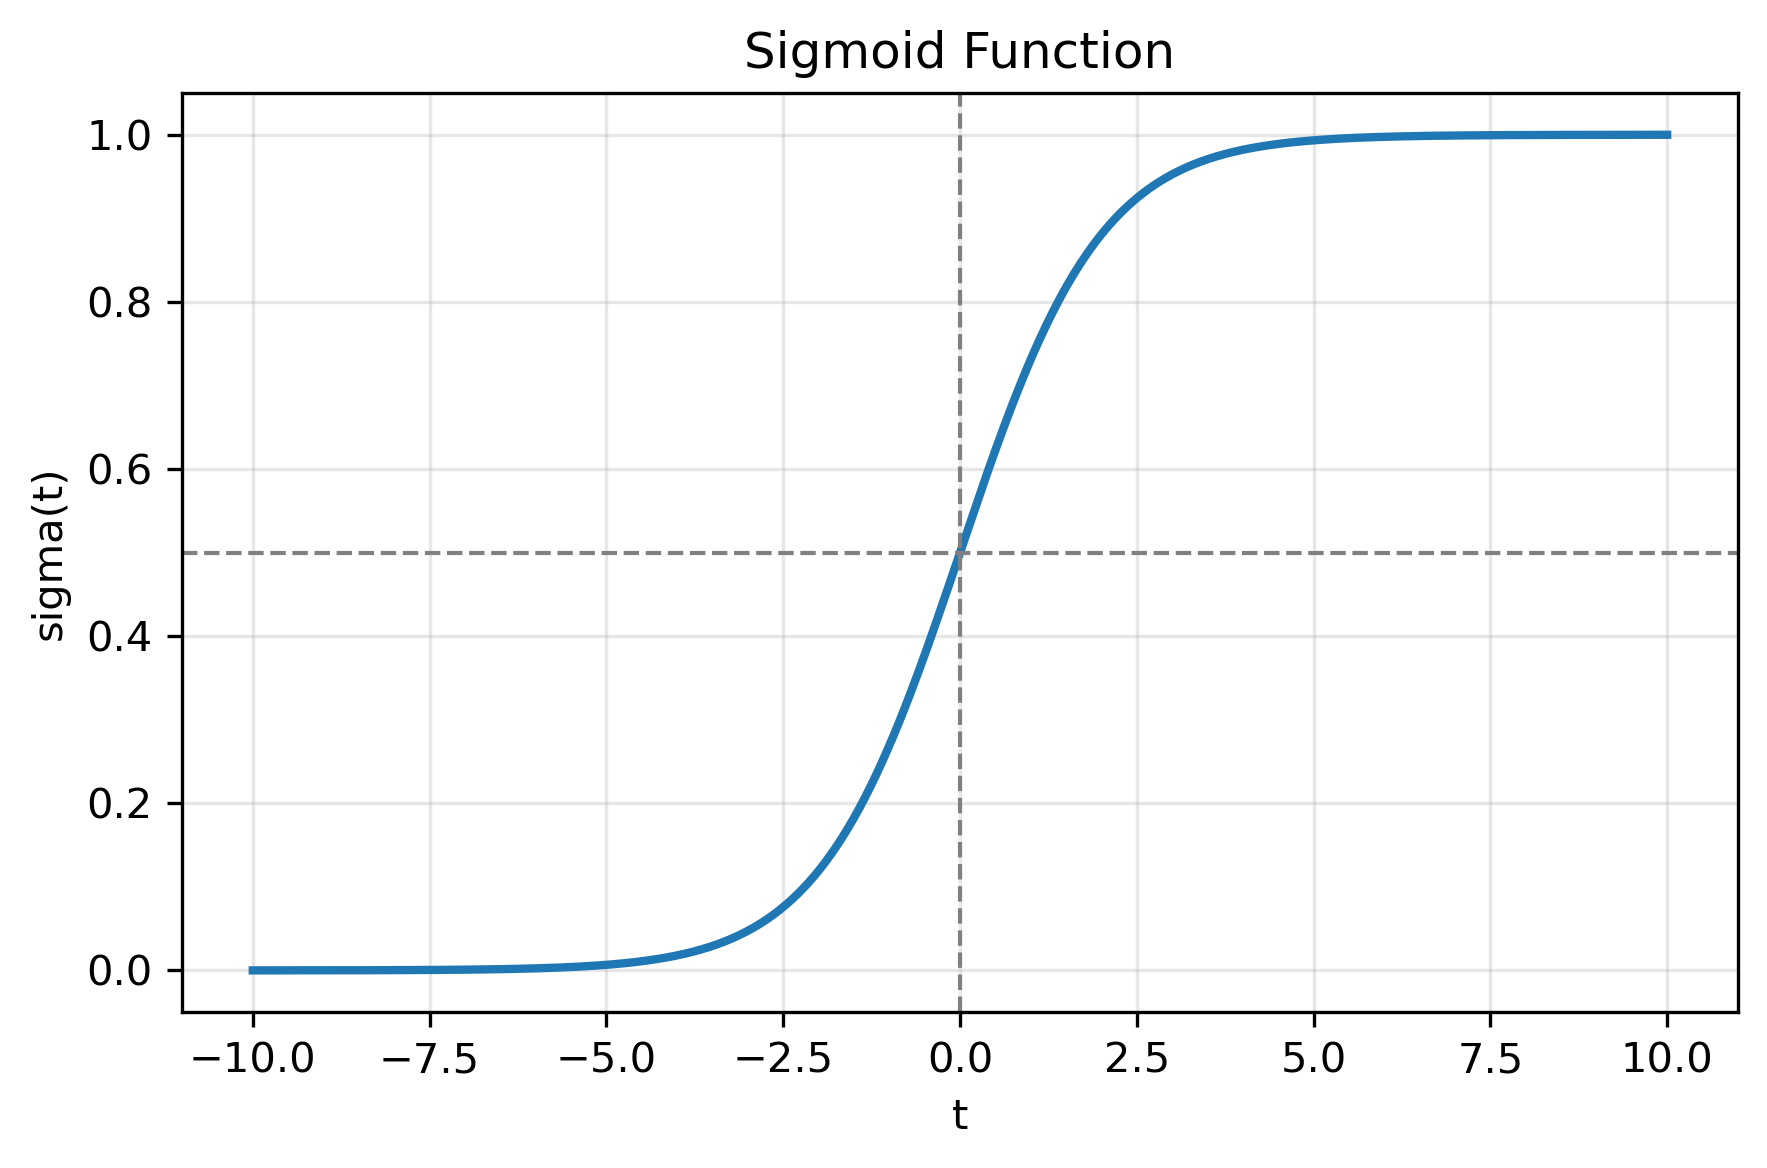
\includegraphics[width=0.65\linewidth]{sigmoid_curve.png}
  \caption{Sigmoid function $\sigma(t)=1/(1+e^{-t})$.}
  \label{fig:sigmoid}
\end{figure}

\begin{figure}[H]
  \centering
  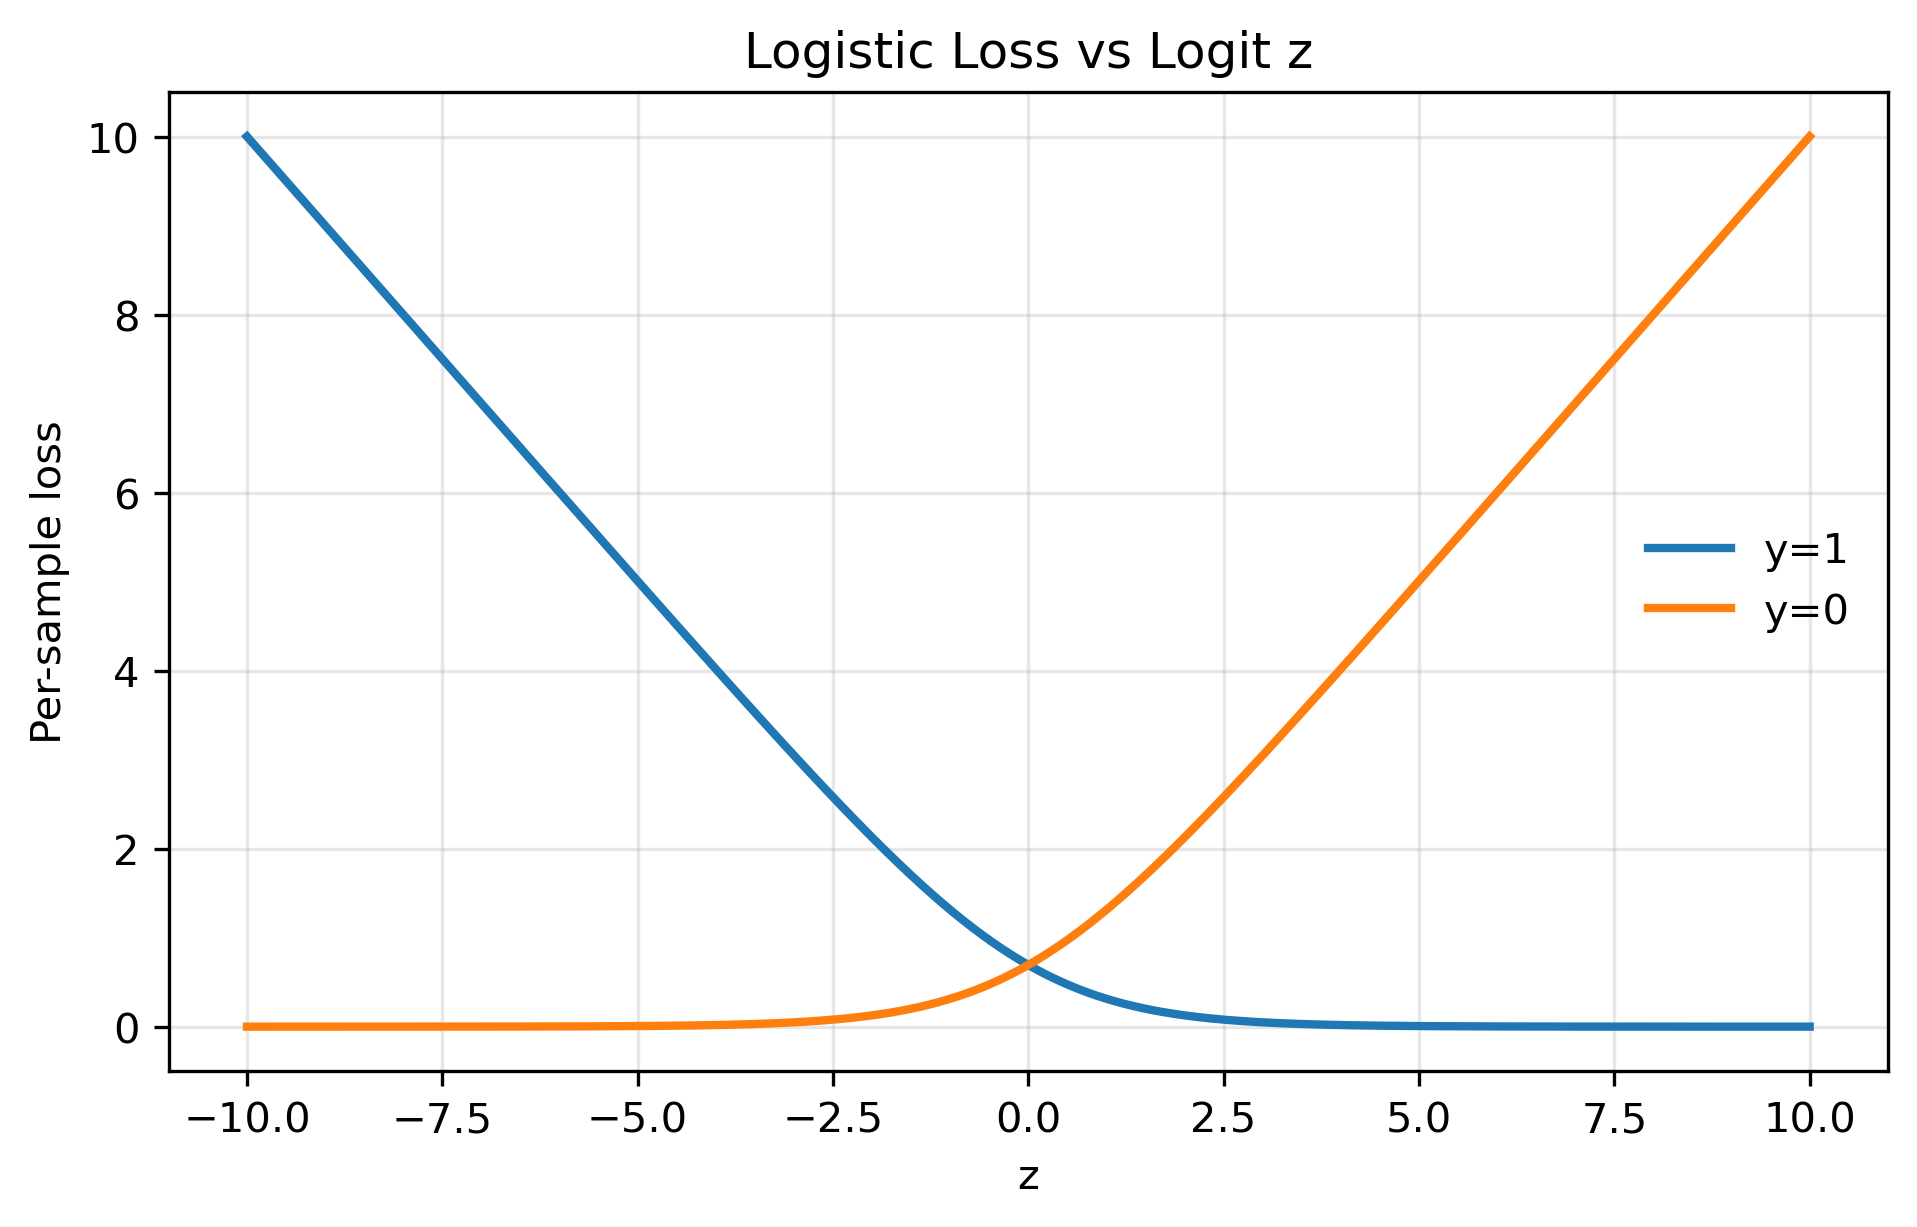
\includegraphics[width=0.7\linewidth]{logistic_loss_curves.png}
  \caption{Binary cross-entropy per-sample loss versus logit $z$ for $y=0$ and $y=1$.}
  \label{fig:loss}
\end{figure}

\begin{figure}[H]
  \centering
  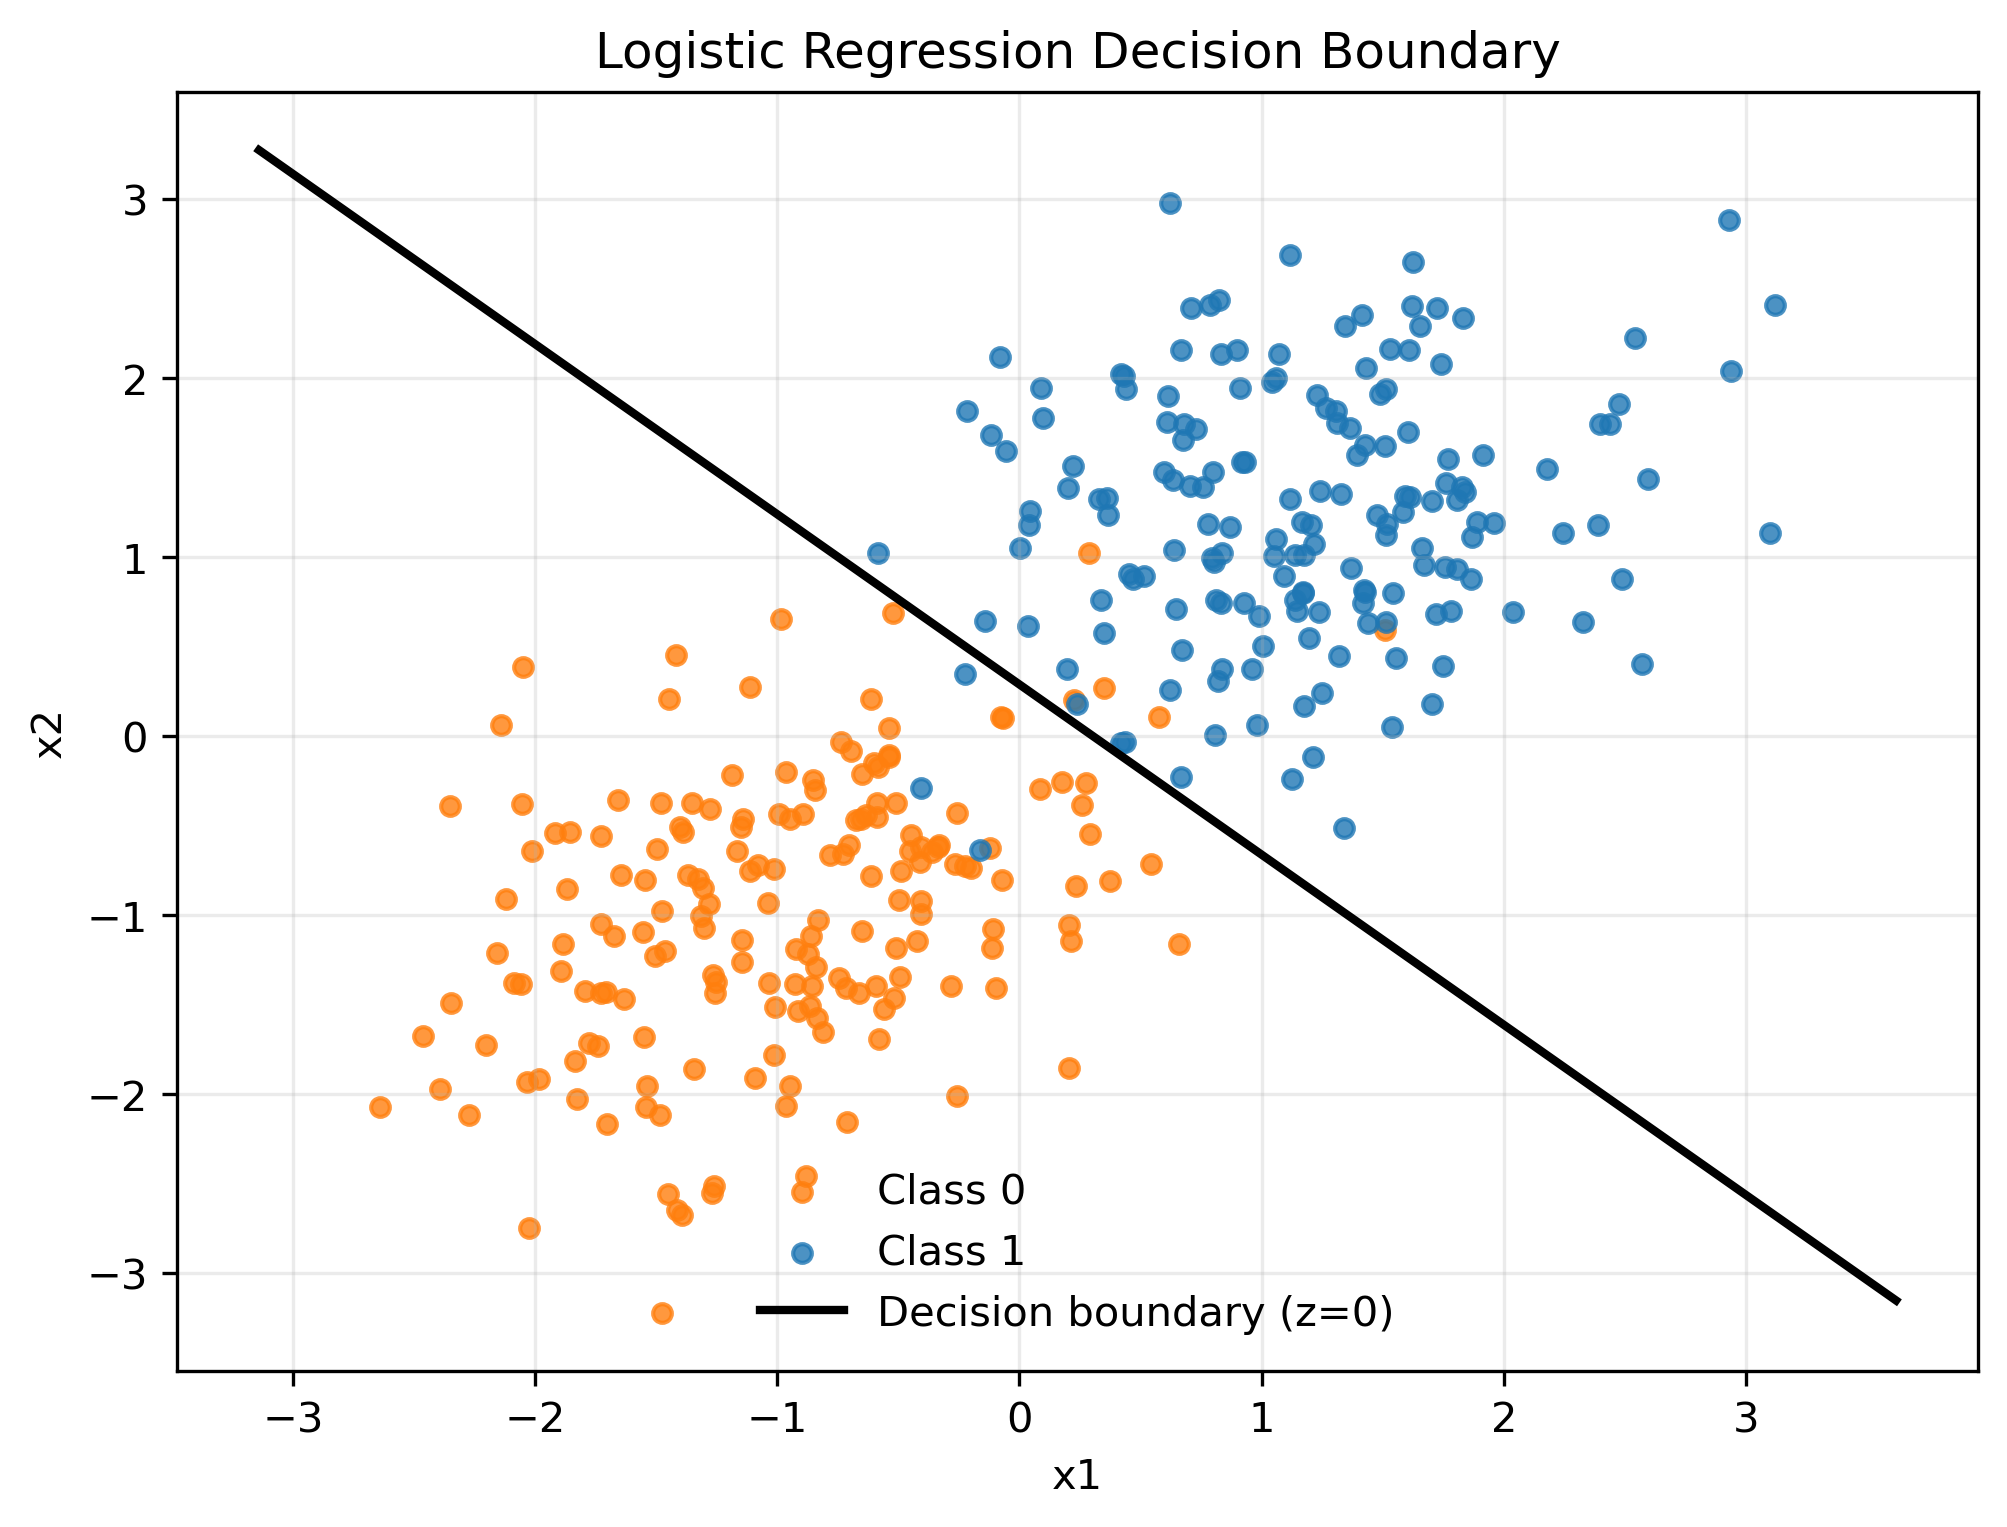
\includegraphics[width=0.75\linewidth]{decision_boundary.png}
  \caption{Synthetic 2D data and learned logistic regression decision boundary.}
  \label{fig:boundary}
\end{figure}

\begin{figure}[H]
  \centering
  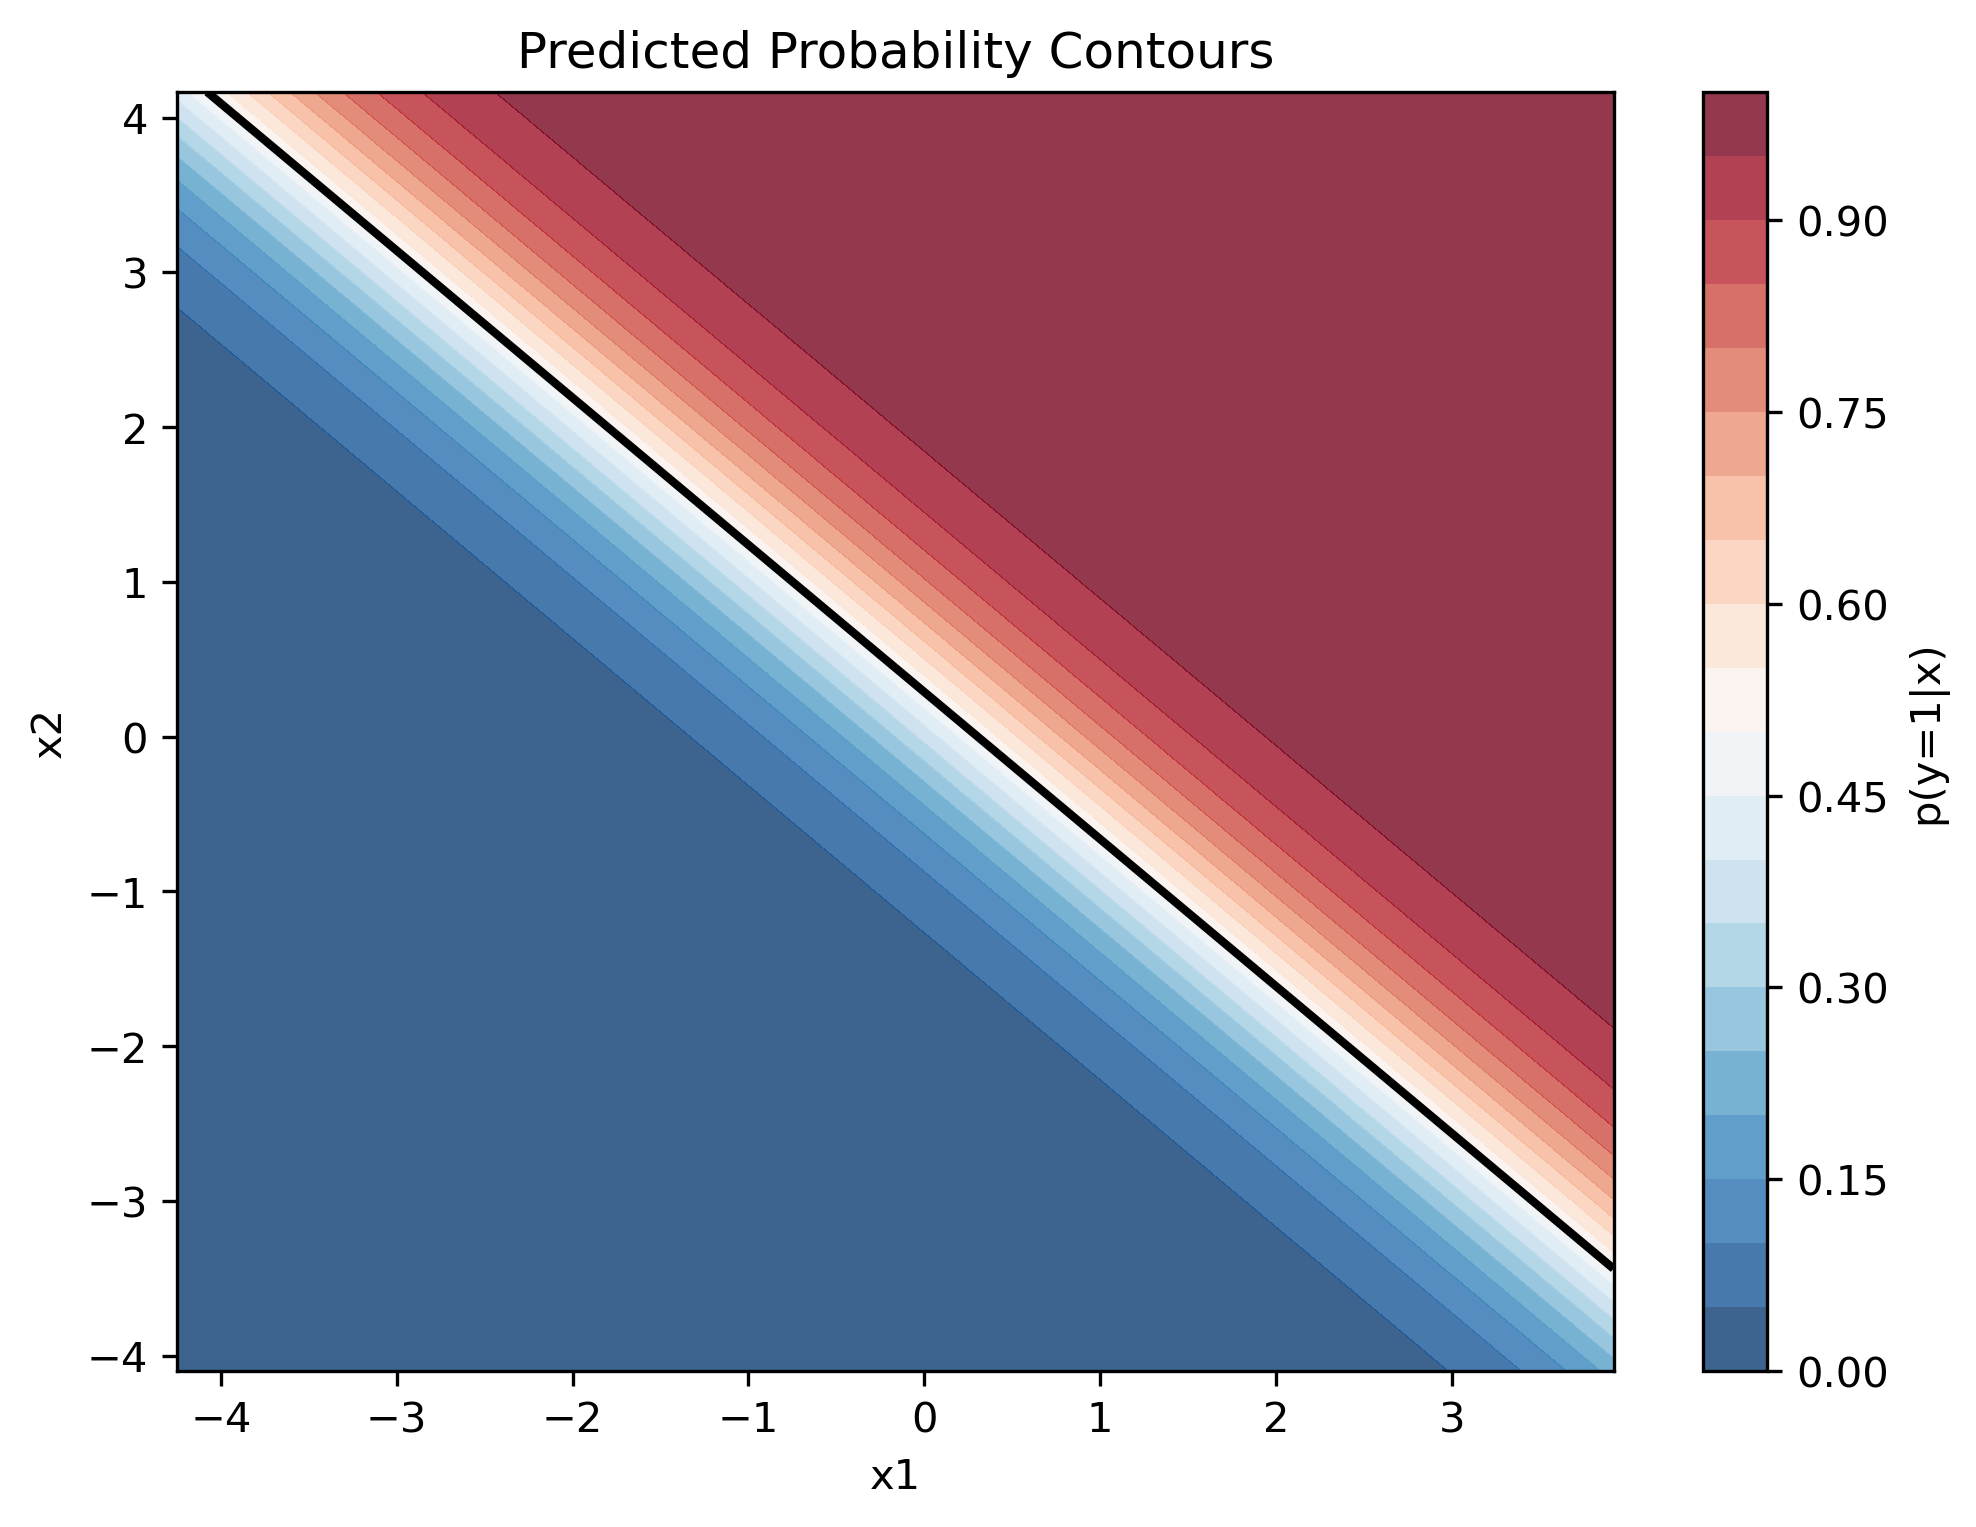
\includegraphics[width=0.75\linewidth]{probability_contours.png}
  \caption{Predicted probability contours $p(y=1\mid \bm{x})$ on a grid.}
  \label{fig:contours}
\end{figure}

\begin{figure}[H]
  \centering
  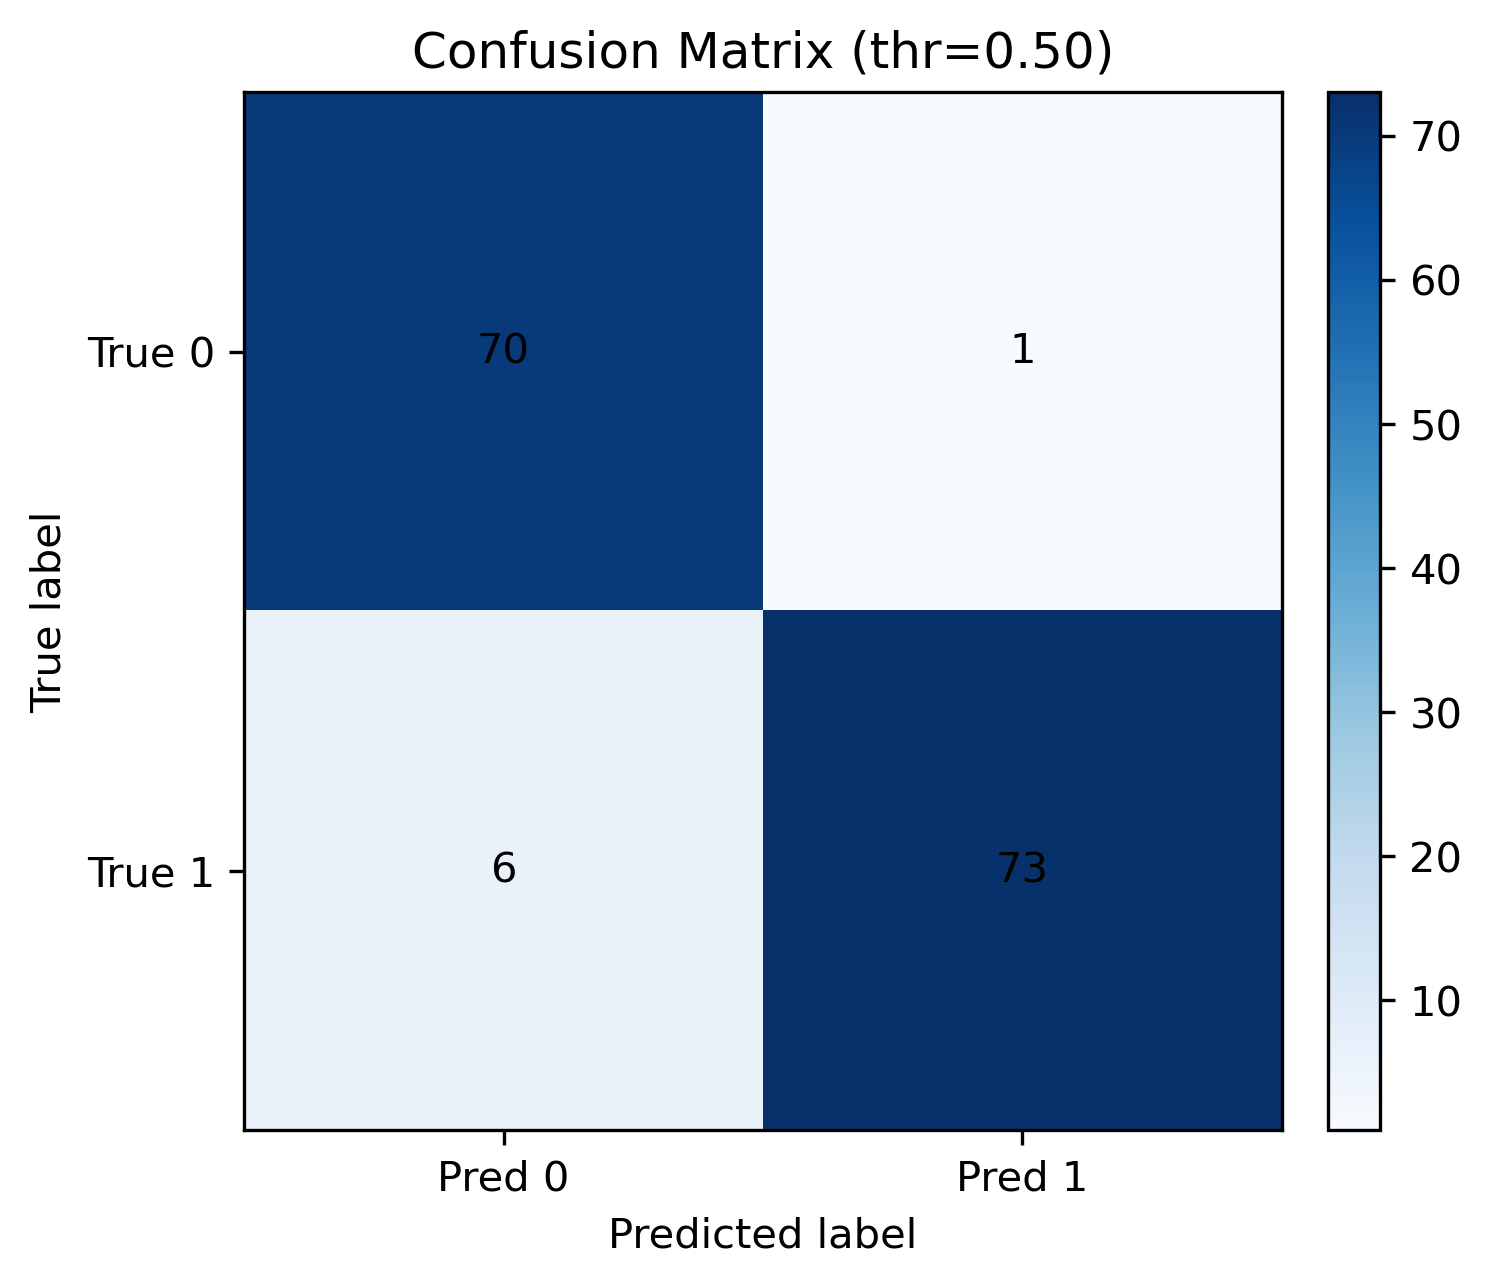
\includegraphics[width=0.55\linewidth]{confusion_matrix.png}
  \caption{Confusion matrix on a held-out split at threshold 0.5.}
  \label{fig:confusion}
\end{figure}

\FloatBarrier

\section{Summary}
Logistic regression provides a simple, interpretable, and effective classifier for many problems. Its probabilistic nature, convex training objective, and linear decision boundary make it a staple in the machine learning toolbox, often serving as a strong baseline.

\end{document}

